\chapter{Kajian Pustaka}

Pada bab ini penulis akan menjelaskan teori yang digunakan selama pengerjaan tugas akhir.

\section{PISA}

\textit{Programme for International Student Assessment} adalah sebuah program yang dilakukan tiga tahun sekali oleh \textit{The Organization for Economic Co-operation and Development}(OECD) dengan tujuan untuk membuat data yang dapat dibandingkan yang akan memungkinkan negara-negara memperbaiki kebijakan dan hasil pendidikan mereka \cite{Pisa1}. Siswa yang dijadikan \textit{sample} pada PISA berumur 15 tahun, hal ini dilakukan karena mereka berada pada akhir pendidikan wajib. Hal yang diujikan dalam PISA berupa matematika, sains, dan membaca.

\section{Sudoku}

Sudoku berasal dari kata \textit{Sūji wa dokushin ni kagiru} yang berarti angkanya harus tunggal \cite{SATPy3}. Sudoku dipopulerkan di jepang oleh \textit{Nikoli in the paper Monthly Nikolist} pada April 1984. Sudoku adalah suatu \textit{puzzle} (teka-teki) yang direpresentasikan oleh sebuah matriks (\textit{array}
dua dimensi) berukuran ${n^2 \times n^2}$  yang dibangun dari ${n^2}$ dengan submatriks (atau blok)
yang berukuran ${n \times n}$. Sudoku merupakan \textit{puzzle}
yang biasanya dimainkan oleh satu orang.  Pada
awal permainan, terdapat beberapa sel yang telah terisi yang disebut dengan pemberian
(\textit{givens}). Untuk menyelesaikan permainan ini, seorang pemain harus mengisi setiap sel yang
belum terisi dengan angka di antara 1 sampai
$n^2$ sedemikan sehingga setiap baris, setiap kolom,
dan setiap blok (submatriks berukuran $n \times n$) memuat tepat satu bilangan di antara 1 sampai $n^2$. Biasanya suatu sudoku didesain agar tepat memiliki satu kemungkinan solusi. Hal
ini juga mengakibatkan sudoku dapat diselesaikan hanya dengan mengandalkan penalaran
yang sederhana. Pengisian suatu sel dapat dilakukan dengan meninjau kemungkinan dari
isi sebuah sel.

\subsection{Sejarah Sudoku}

Sebelum sudoku modern berkembang. \textit{Puzzle latin square} terlebih dahulu berkembang yang di repretasikan oleh sebuah matriks berukuran ${n \times n}$ yang memiliki angka ${1 hingga n}$ yang harus diisi oleh pemain. untuk menyelesakain \textit{puzzle }setiap baris dan kolom pada \textit{latin square} harus memiliki nilai angka yang berbeda. \textit{Latin square} pertama kali diciptakan oleh Euler pada tahun 1783 \cite{Unk1}. Pada 19 November 1892 \textit{ Le Siècle} sebuah surat kabar di perancis mempublikasikan \textit{magic square} yaitu sebuah teka-teki  yang di repretasikan oleh sebuah matriks berukuran ${9 \times 9}$ yang memiliki dua buah submatriks berukuran ${3 \times 3}$. Tujuan dari \textit{magic square} adalah pemain mengisi baris dan kolom sehingga nilai penjumlahan setiap baris dan kolom itu sama. 

\begin{figure}[H]
	\begin{centering}
		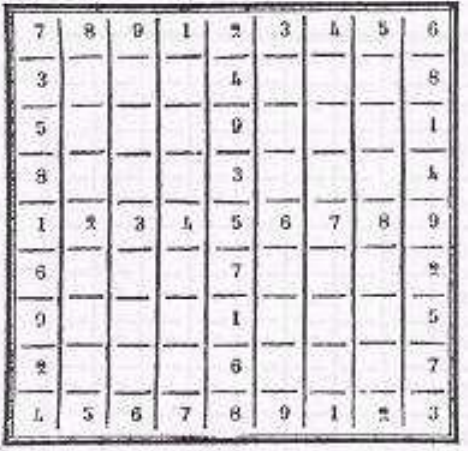
\includegraphics[scale=0.7]{gambar/magicSquare}
		
		\caption{Benduk \textit{magic square}. (gambar diambil dari \cite{SATPy4})}
	\end{centering}
\end{figure}

Sudoku modern sendiri lahir dari  Howard Garns yang dipublikasikan di \textit{Dell Magazines} pada 1979 \cite{SATPy5}.	

\subsection{Penyelesaian Sudoku}

Dalam menyelesaikan sudoku terdapat banyak cara. Namun salah satu cara yang paling efektif adalah dengan berikut: 

\subsubsection{Memeriksa Baris, Kolom, dan Blok}

Pada sudoku dengan ukuran $9 \times 9$ Untuk menyelesaikan sudoku pemain tidak boleh menaruh angka yang sama di baris, kolom, atau blok ${3 \times 3}$.

\begin{figure}[H]
	\begin{centering}
		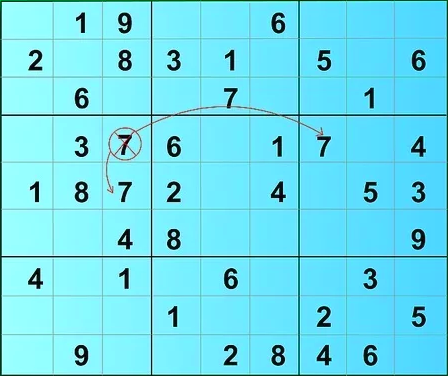
\includegraphics[scale=0.7]{gambar/solve1}
		
		\caption{7 tidak mungkin pada sel tersebut. (gambar diambil dari \cite{Sud12})}
	\end{centering}
\end{figure}

\subsubsection{Menemukan \textit{Define}}

\textit{Define} adalah angka yang pasti ada pada sel itu. \textit{Define} dipengaruhi oleh \textit{given} suatu sudoku. Untuk mempermudah menemukan \textit{define} pemain memulai mencarinya dari angka 1 lalu menarik sebuah garis dari setiap \textit{given} bernilai 1. Ketika hanya ada satu sel tersisa pada sebuah blok maka sel itu memiliki \textit{Define} angka 1. 

\begin{figure}[H]
	\begin{centering}
		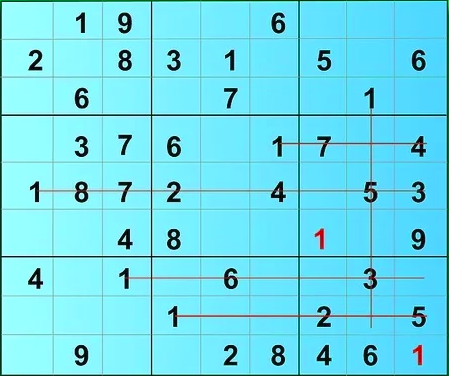
\includegraphics[scale=0.7]{gambar/solve2}
		
		\caption{Menemukan \textit{define}. (gambar diambil dari \cite{Sud12})}
	\end{centering}
\end{figure}

Ulangi proses yang sama hingga angka 9.

\begin{figure}[H]
	\begin{centering}
		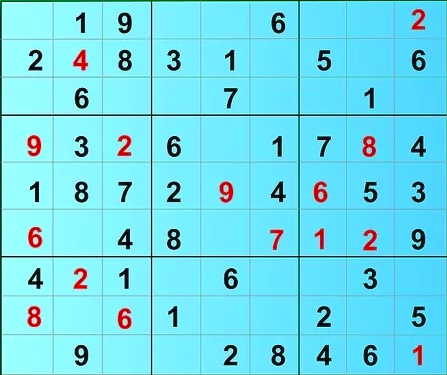
\includegraphics[scale=0.7]{gambar/solve3}
		
		\caption{Semua \textit{define} ditemukan. (gambar diambil dari \cite{Sud12})}
	\end{centering}
\end{figure}



\subsubsection{\textit{Backtrack} Ketika Mengalami Kemacetan}

Ketika pemain mengalami kemacetan dalam mengerjakan sudoko. Hal ini terjadi karena pemain salah  memasukkan angka pada sel diluar \textit{define}. Salah satu caranya adalah dengan memberi catatan untuk setiap blok dengan angka yang mungkin berada  pada sel tersebut.



\begin{figure}[H]
	\begin{centering}
		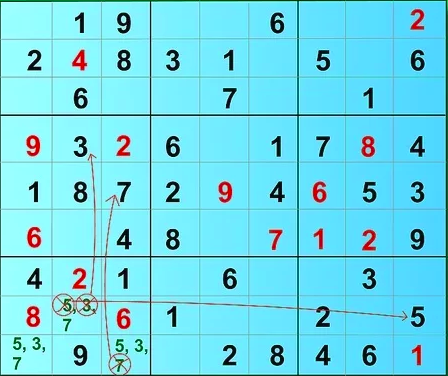
\includegraphics[scale=0.7]{gambar/solve4}
		
		\caption{Catatan yang berisi setiap kemungkinan angka. (gambar diambil dari \cite{Sud12})}
		\end{centering}
		\end{figure}
		


\section{Metode Formal}

Metode formal adalah teknik yang digunakan untuk memodelkan suatu
sistem yang kompleks \cite{huth2004logic}. Metode formal dapat digunakan untuk mengembangkan
sebuah aplikasi baik itu perangkat lunak atau perangkat keras. Pada
masa spesifikasi, metode formal dapat digunakan untuk memberikan gambaran
dari sistem yang akan dikembangkan sedetail yang diinginkan. Metode
formal dapat digunakan untuk memandu kegiatan pengembangan selanjutnya
dan dapat digunakan untuk memverifikasi bahwa pra-syarat untuk sistem yang
dikembangkan telah lengkap dan dapat dilanjutkan ke tingkat selanjutnya.

\section{Pengujian Kotak Hitam}

Pengujian kotak hitam adalah teknik pengujian yang tidak memerlukan pengetahuan kode dari aplikasi \cite{TEST1}. Penguji biasanya melakukan pengujian kotak hitam melalui antarmuka pengguna dari aplikasi dengan diberikan \textit{test case} masukan dan menganalisa keluaran dari aplikasi.

\section{Logika Proposisi}

Logika proposisi adalah bahasa formal untuk memodelkan situasi yang kita sehingga kita dapat memberi alasan tentang hal itu secara formal \cite{huth2004logic}. Logika proposisi terdiri dari sebuah nilai kebenaran dari proposisinya.

Operator yang digunakan pada logika proposisi adalah sebagai berikut

\begin{itemize}
	\item Konjungsi(dan) pada operator ini kedua proposisi yang dihubungkan harus bernilai benar agar formula bernilai \textit{true}
	. Operator ini dilambangkan dengan $\wedge$.
	\item Disjungsi(atau) pada operator ini salah satu proposisi yang dihubungkan harus bernilai benar agar formula bernilai \textit{true}. Operator ini dilambangkan dengan $\lor$ 
	\item Negasi(tidak) pada operator ini suatu proposisi akan memiliki nilai sebaliknya dari sebuah proposisi. Operator ini dilambangkan dengan $\neg$
	\item Implikasi(jika-maka) pada operator ini digunakan untuk merepresantisakan kata \textquotedblleft jika p maka q\textquotedblright sebuah formula akan bernilai \textit{false} jika nilai p benar dan nilai q salah. Operator ini dilambangkan dengan $\to$. 
	\item Biimplikasi(jika dan hanya jika)pada operator ini suatu formula hanya akan bernilai \textit{true} jika kedua proposisinya memiliki nilai kebenaran yang sama. Operator ini dilambangkan dengan $\leftrightarrow$
	
\end{itemize}

\section{\textit{Satisfiability Problem}(SAT)}

Masalah SAT (SAT \textit{problem}) adalah salah satu masalah penting dalam logika komputasional \cite{huth2004logic}. Dalam pengerjaannya SAT berfokus pada membuktikan sebuah klausa \textit{satisfiable} sehingga SAT berfokus pada menemukan sebuah model yang membuat klausa tersebut \textit{satisfiable}. Jika tidak ditemukan sebuah model yang membuat klausa tersebut \textit{satisfiable} maka klausa tersebut \textit{unsatisfiable}. Masalah SAT merupakan masalah NP-complete, hingga saat ini tidak
terdapat algoritma yang efisien untuk memecahkan masalah tersebut. 

\subsection{Penyelesaian Sudoku Dengan SAT}
Sudoku memiliki beberapa aturan contohnya untuk sudoku berukuran  $9 \times 9$ yaitu :

\begin{enumerate}
	\item Setiap baris memuat bilangan antara 1 hingga 9.
	\item Setiap kolom memuat bilangan antara 1 hingga 9.
	\item Setiap submatriks atau blok $3 \times 3$
	 memuat bilangan antara 1 hingga 9.
	\item Setiap sel memuat tepat satu bilangan antara 1 hingga 9.
\end{enumerate}

Dari aturan-aturan tersebut akan ditranslasikan menjadi bentuk CNF lalu digunakan pada SAT \textit{solver}. Dengan aturan yang telah ditranslasikan dalam CNF sebagai berikut:

\begin{enumerate}
	\item Setiap baris memuat bilangan antara 1 
	hingga 9 : 
	
	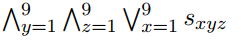
\includegraphics[scale=1]{gambar/rule1}
	
	\item Setiap kolom memuat bilangan antara 1 hingga 9 : 
	
	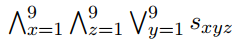
\includegraphics[scale=1]{gambar/rule2}
	
	\item Setiap submatriks atau blok $3 \times 3$
	memuat bilangan antara 1 hingga 9 : 
	
	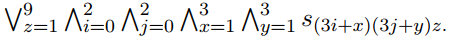
\includegraphics[scale=1]{gambar/rule3}
	
	\item Setiap sel memuat tepat satu bilangan antara 1 hingga 9 : 
	
	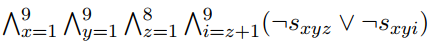
\includegraphics[scale=1]{gambar/rule4}
	
\end{enumerate}


\section{\textit{Waterfall Design}}

\textit{Waterfall} atau air terjun adalah model yang diperkenalkan oleh Dr.
Winston W. Royce pada tahun 1970. Model ini menuntun pengembang untuk
melakukan pengembangan perangkat lunak yang akan dibangun secara sistematis
dan mempunyai keterkaitan antara prosesnya. dalam arti tahapan proses
berikutnya tidak akan dapat di wujudkan jika tahapan sebelumnya tidak
terselasaikan.

Ada dua langkah penting yang harus ada dalam pembuatan perangkat lunak. pertama ialah analisis lalu di ikuti oleh \textit{coding}, jika di bagi akan menjadi beberapa tahap yang spesifik yaitu \textit{System
Requirements} $\to$ \textit{Software Requirements} $\to$ \textit{Analysis} $\to$ \textit{Program Design} $\to$ \textit{Coding} $\to$ \textit{Testing} \cite{royce1987managing}. 

